\documentclass[11pt]{article}
\title{\textbf{Horns unit}}
\author{https://github.com/heptagons/meccano/units/horns}
\date{}

\usepackage{../../meccano}
\usepackage{tikz}
\usetikzlibrary{calc}

\begin{document}

\maketitle
\begin{abstract}
Horns unit is a group of seven meccano\meccanoref strips intended to build polygons.
\end{abstract}

\begin{figure}[h]
\centering
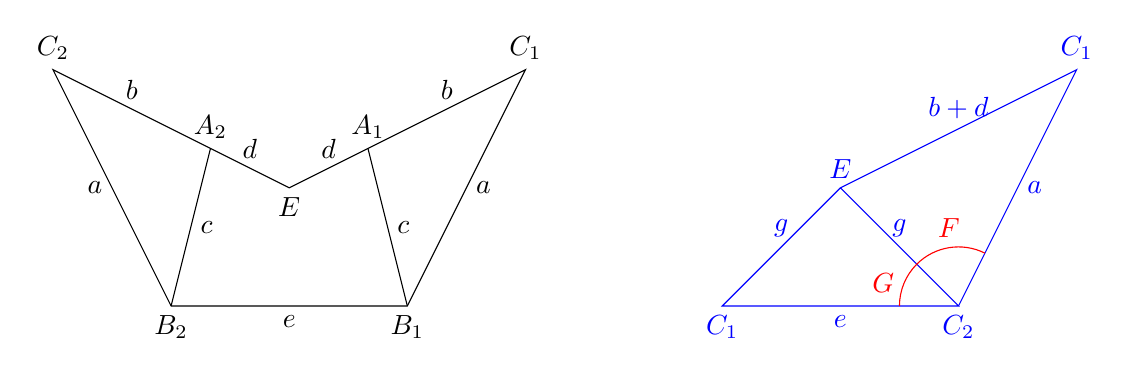
\begin{tikzpicture}
 \begin{scope}[scale=0.5]
  \draw[black] (0,0)
  -- node[below] {$e$} ++(6,0) node[below] {$B_1$}
  -- node[below,right] {$a$} ++(3,6) node[above] {$C_1$}
  -- node[above] {$b$} ++(-4,-2) node[above] {$A_1$}
  -- node[above] {$d$} ++(-2,-1) node[below] {$E$}
  -- node[above] {$d$} ++(-2,1) node[above] {$A_2$}
  -- node[above] {$b$} ++(-4,2) node[above] {$C_2$}
  -- node[below,left] {$a$} ++(3,-6) node[below] {$B_2$}
  -- cycle;
  \draw[black] (6,0) --++ (-1,4) node[midway,right] {$c$};
  \draw[black] (0,0) --++ (+1,4) node[midway,right] {$c$};

  \draw[blue] (20,0)
  -- node[below,right] {$a$} ++(3,6) node[above] {$C_1$}
  -- node[above] {$b+d$} ++(-6,-3) node[above] {$E$}
  -- node[above] {$g$} ++(-3,-3) node[below] {$C_1$}
  -- node[below] {$e$} ++(6,0) node[below] {$C_2$}
  -- node[above] {$g$} ++(-3,+3);
  
  \draw[red] (20,0)+(-1.5,0) 
   arc (180:135:1.5) node[midway,above,left] {$G$}
   arc (135:atan(2):1.5) node[midway,above] {$F$};

 \end{scope}
\end{tikzpicture}
\caption{Horns units. Has seven strips: Two of length $a$, two of length $b+d$,
two of length $c$ and one of length $e$.
We expect to build polygons with internal angle $C_1B_1B_2$
and perimeter including segments $a,e,a$.}
\end{figure}

\section{Algebra}
Angle = $\angle{C_1B_1B_2}$.

\end{document}
